%%%%%%%%%%%%%%%%%%%%%%%%%%%%%%%%%%%%
% Section: Sponge & Duplex Constructions
%%%%%%%%%%%%%%%%%%%%%%%%%%%%%%%%%%%%
\section{Sponge \& Duplex Constructions}
\begin{frame}
\frametitle{Sponge Construction}
\begin{itemize}
  \item Gaining popularity recently
  \begin{itemize}
    \item Sponge-based \Keccak hash function won SHA-3 competition
  \end{itemize}
  \item Provides way to generalize hash functions to have arbitrary length output
  \item Allows \textbf{many} other uses outside of hashing
  \item Built from underlying iterated \emph{sponge permutation} $f$
\end{itemize}
\end{frame}

\begin{frame}
\frametitle{Sponge Construction}
\begin{figure}[ht]
\centering
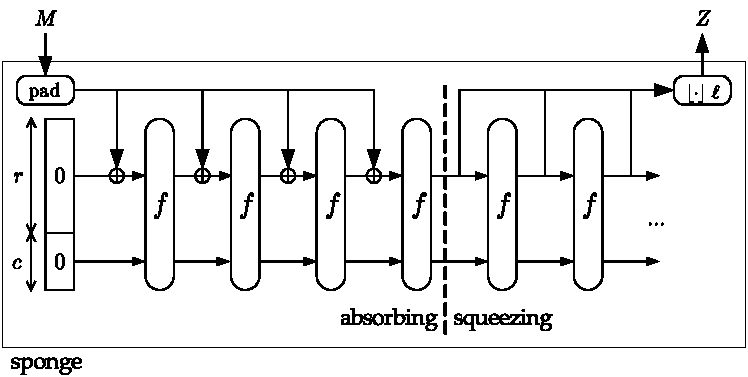
\includegraphics[width=\textwidth]{img/Sponge.pdf}
\caption{The sponge construction $\mathbf{sponge}[f,\mathbf{pad},r]$ \cite{Bertoni2011_SpongeFunctions}}
\label{fig:Sponge}
\end{figure}
\end{frame}

\begin{frame}
\frametitle{Sponge Parameters}
\begin{itemize}
  \item State size / width, $b = r + c$
  \item Rate, $r$:
  \begin{itemize}
    \item Exposed portion of state - \emph{outer state}
    \item Absorb and squeeze in $r$-bit blocks
    \item Speed is mostly dependent on $r$
  \end{itemize}
  \item Capacity, $c$:
  \begin{itemize}
    \item Hidden portion of state - \emph{inner state}
    \item Security is mostly dependent on $c$
  \end{itemize}
\end{itemize}
\end{frame}

\begin{frame}
\frametitle{Simplified Sponge}
\begin{itemize}
  \item Ignore padding 
  \item May be done at higher level in system
  \item Focus more / all design effort on underlying permutation
\end{itemize}
\end{frame}

\begin{frame}
\frametitle{Sponge Applications}
\begin{enumerate}
  \item \textbf{Hashing}
  \begin{itemize}
    \item Absorb plaintext - long
    \item Squeeze out message digest - short
  \end{itemize}
  \item \textbf{Encryption} 
  \begin{itemize}
    \item Absorb key and IV - short
    \item Squeeze out keystream - long
  \end{itemize}
  \item \textbf{MAC Generation}
  \begin{itemize}
    \item Absorb key then message - long 
    \item Squeeze out MAC - short
  \end{itemize}
  \item \textbf{Others}
  \begin{itemize}
    \item All without changing the overall construction!
  \end{itemize}
\end{enumerate}
\end{frame}

\begin{frame}
\frametitle{Sponge for AE?}
\begin{itemize}
  \item Sponge can do encryption and MAC generation
  \item ...so can it do authenticated encryption?
  \item Yes! But:
  \begin{itemize}
    \item No intermediate tags
    \item State not maintained between calls
    \item Would require re-initialization between calls
  \end{itemize}
  \item Modify it slightly to get much more flexibility
\end{itemize}
\end{frame}

\begin{frame}
\frametitle{Duplex Construction}
\begin{itemize}
  \item Maintains state between calls
  \item Construct a duplex object $\mathrm{D}$
  \item Make calls to $\mathrm{D}.\mathbf{duplexing}$
  \item Arbitrary length inputs and outputs, including length zero
  \item \emph{Blank call}: no input provided
  \item \emph{Mute call}: no output requested
\end{itemize}
\end{frame}

\begin{frame}
\frametitle{Duplex Illustrated}
\begin{figure}[ht]
\centering
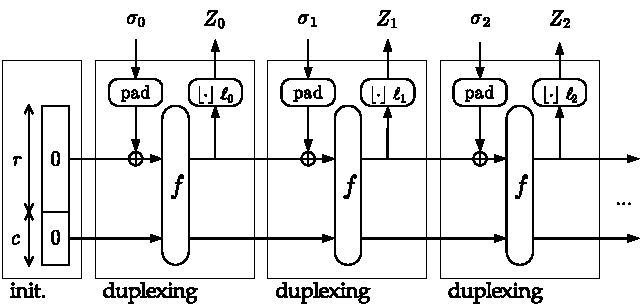
\includegraphics[width=\textwidth]{img/Duplex.pdf}
\caption{The duplex construction $\mathbf{duplex}[f,\mathbf{pad},r]$ \cite{Bertoni2011_SpongeFunctions}}
\label{fig:Duplex}
\end{figure}
\end{frame}

\begin{frame}
\frametitle{Duplex Expanded}
\begin{figure}[ht]
\centering
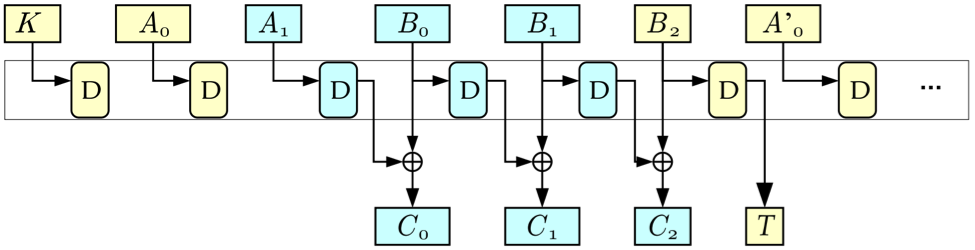
\includegraphics[width=\textwidth]{img/DuplexAE_Expanded.png}
\caption{$K$ = Key, $A$ = Header, $B$ = Body \cite{Bertoni2010_DuplexingSlides}}
\label{fig:DuplexAE_Expanded}
\end{figure}
\end{frame}

\begin{frame}
\frametitle{Duplex for AE}
\begin{enumerate}
  \item Easy to use
  \item Single key required
  \item Single-pass for encryption and authentication
  \item Support for intermediate tags
  \item Support for Additional Authenticated Data (AAD, or headers)
  \item Secure against generic attacks
  \item Ability to trade off speed and security by adjusting $r$
\end{enumerate}
\end{frame}

\begin{frame}
\frametitle{Generic Security}
\begin{itemize}
  \item Duplex construction can be reduced to sponge construction
  \item Sponge construction is secure against \emph{generic attacks}
  \begin{itemize}
    \item Attacks which don't exploit specific properties of $f$
  \end{itemize}
  \item If $f$ is secure, so is the sponge construction it lives in
\end{itemize}
\end{frame}

\begin{frame}
\frametitle{Keyed Sponge Security}
\begin{itemize}
  \item Keyed sponges are more secure than unkeyed \cite{Bertoni2011_SpongeKeyed}
  \item Lower bound by Jovanovic et.~al\ in 2014 \cite{Jovanovic2014_Beyond}:
  \begin{equation*}
  \mathrm{min}(2^{(r+c)/2}, 2^c, 2^{|K|}).
  \end{equation*} 
  \item Allows designers to properly choose $c$ for desired generic security
\end{itemize}
\end{frame}



